\documentclass{beamer}
\usepackage[utf8x]{inputenc}
\usepackage{graphicx}
\usepackage{tikz}
\graphicspath{{./../../img/}}

\usepackage[T1]{fontenc}

\usetheme{TUM}

\title[Research Graph]{Research Graph}

\author[Guerin, Silva, Zimmerer]{Fiona Guerin, Alvaro Silva, Andreas Zimmerer}
\institute{Technical University of Munich}

\date{17 December 2019}

% Customize alert
\setbeamercolor{alerted text}{fg=TUMZusatzfarbeBlau3}
\setbeamerfont{alerted text}{series=\bfseries}

\begin{document}
\maketitle

\begin{frame}{Vision}
    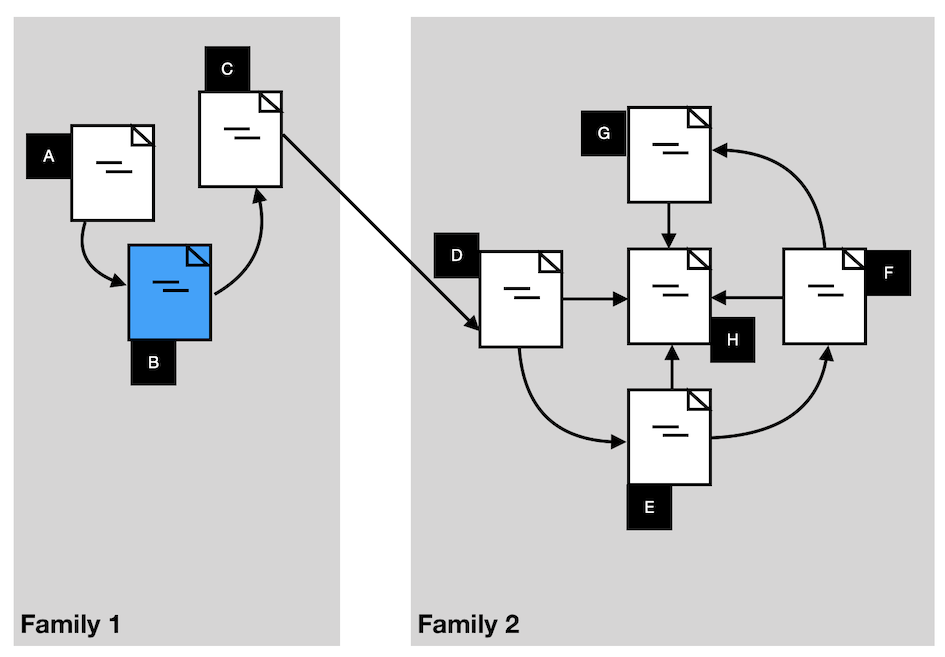
\includegraphics{img_02.png}
\end{frame}

\begin{frame}{Demo}
\url{Link: http://localhost:3000}
\end{frame}

\begin{frame}{Demo: Force-Based Positions}
    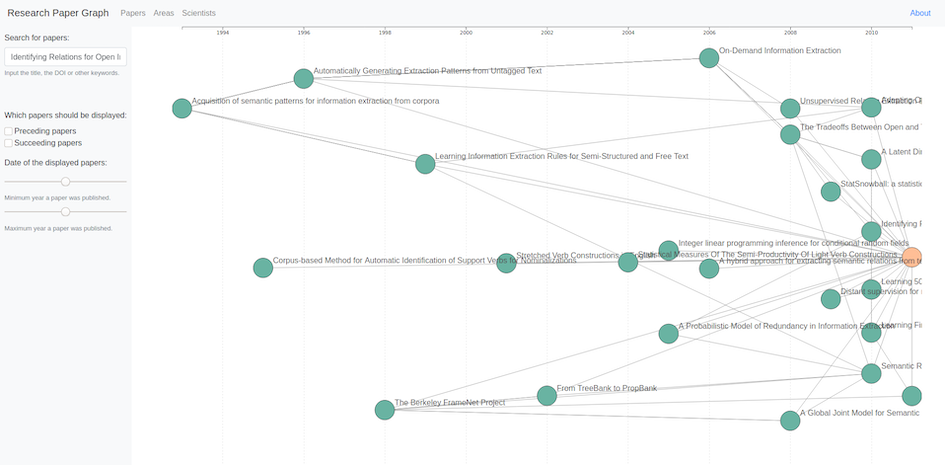
\includegraphics{graph_random_positions.png}
\end{frame}

\begin{frame}{Demo: Computed Positions}
    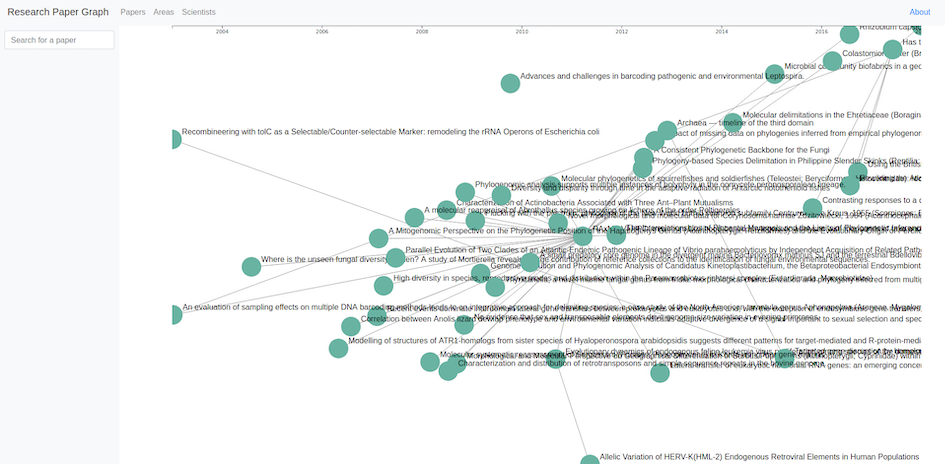
\includegraphics{graph_computed_positions.png}
\end{frame}

\begin{frame}{Architecture}
    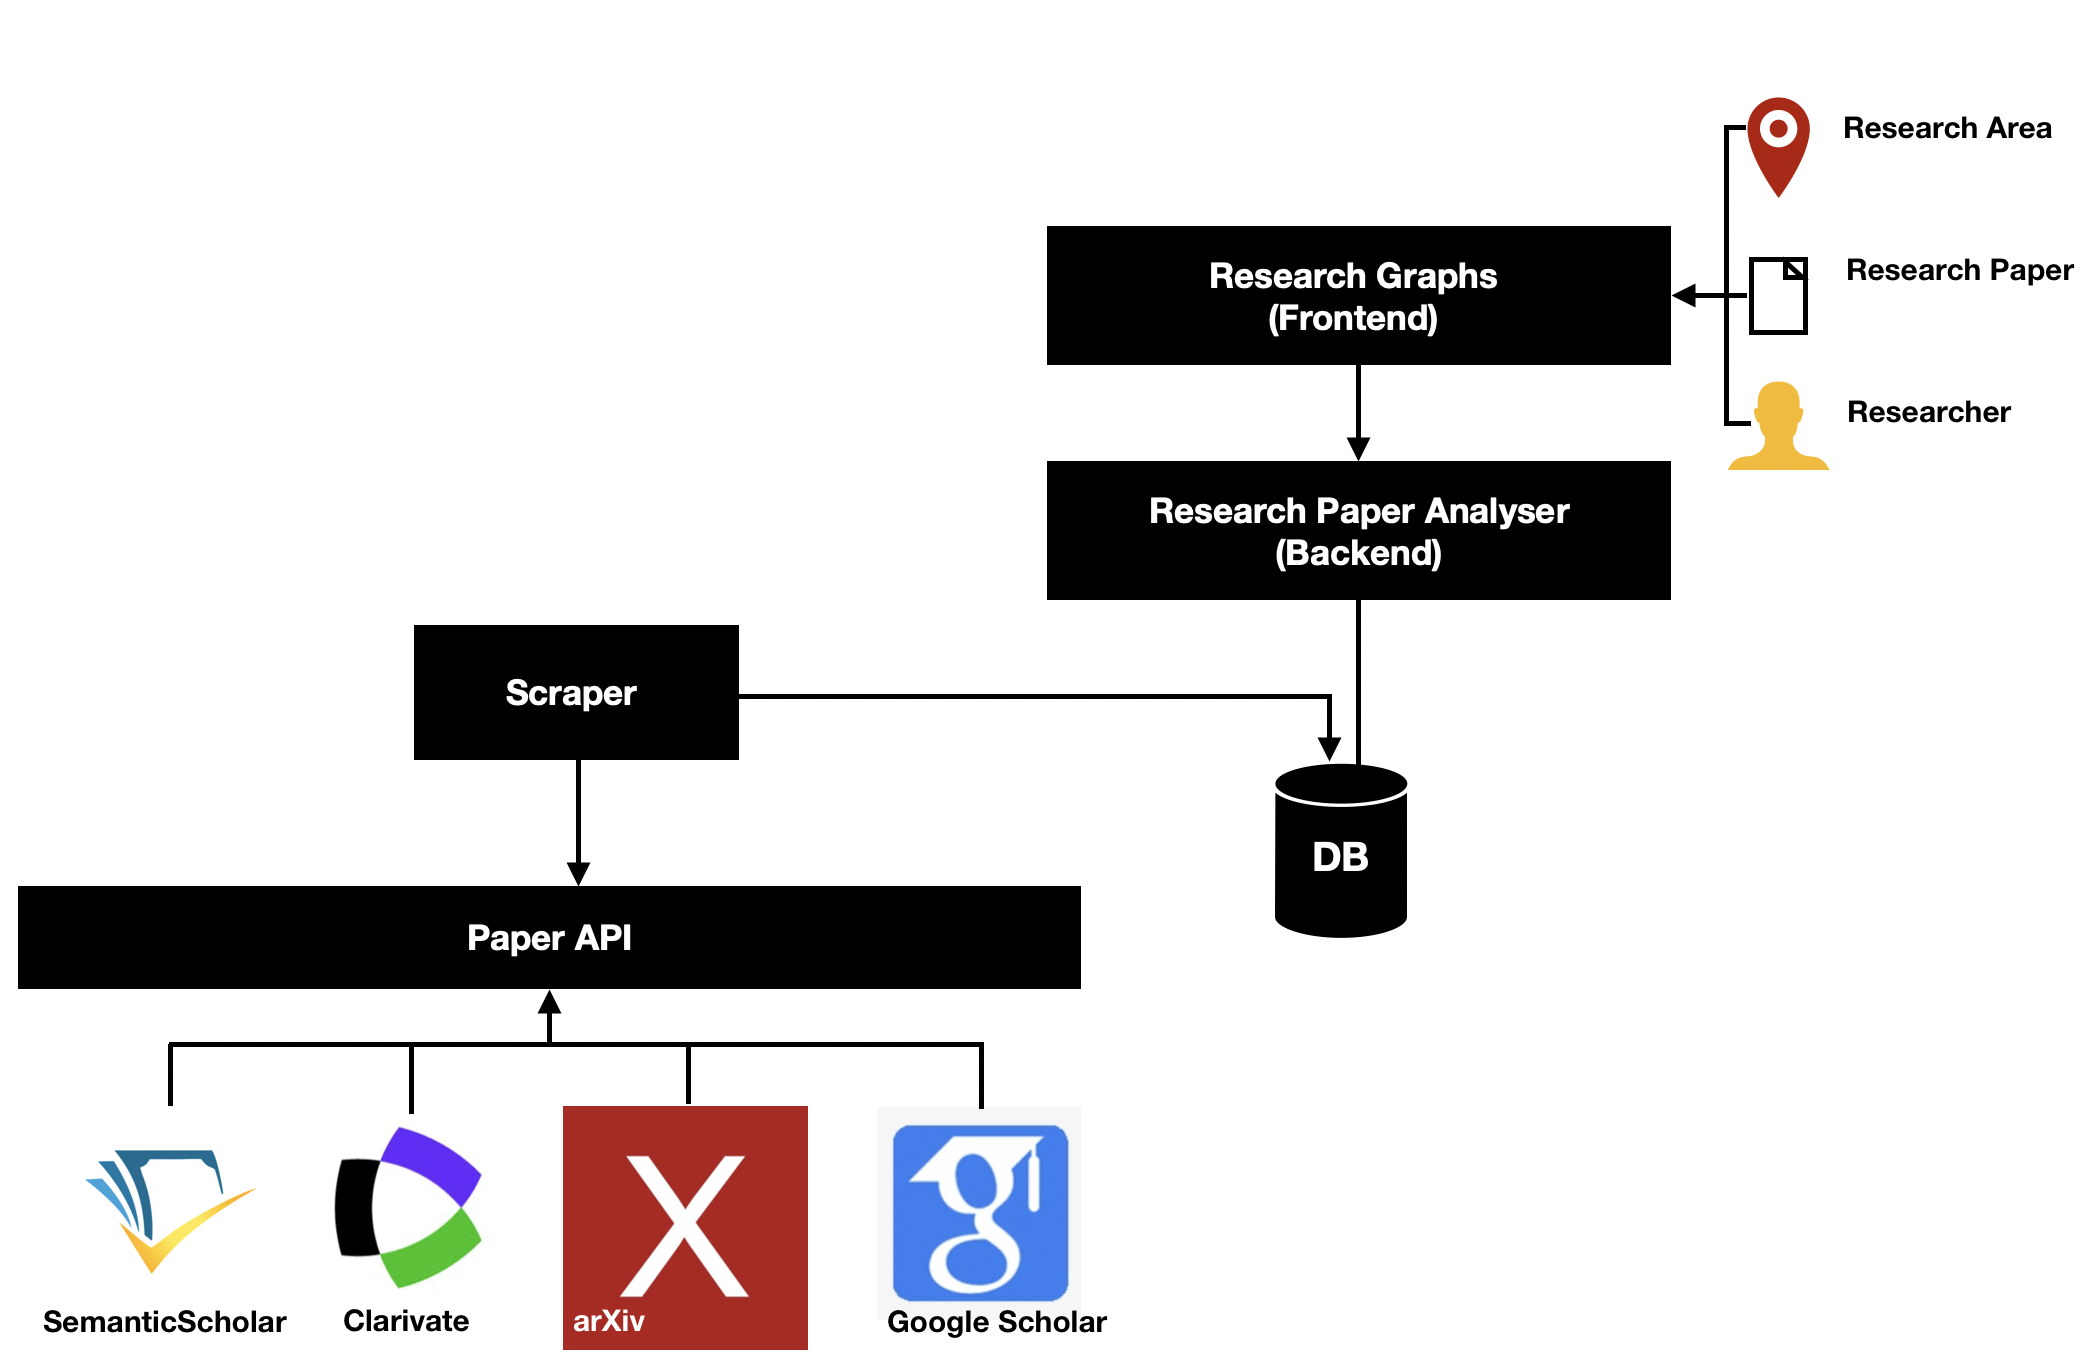
\includegraphics{img_03.png}
\end{frame}

\begin{frame}{Frontend}
    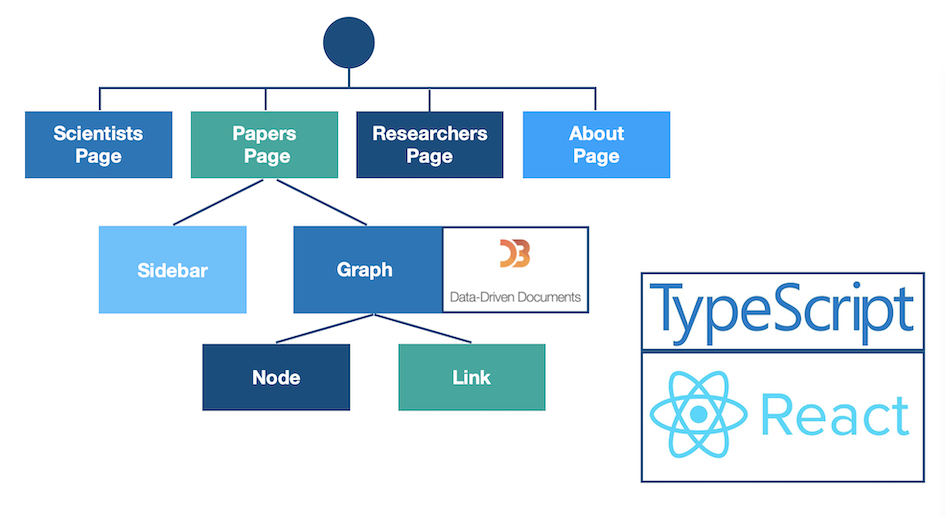
\includegraphics{img_06.png}
\end{frame}

\begin{frame}{Database}
    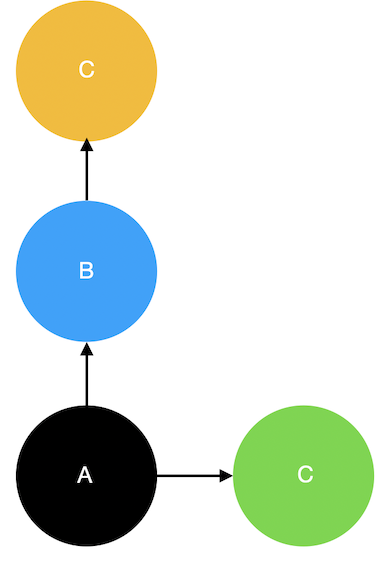
\includegraphics{img_07.png}
\end{frame}

\begin{frame}{Backend and Scraper}
    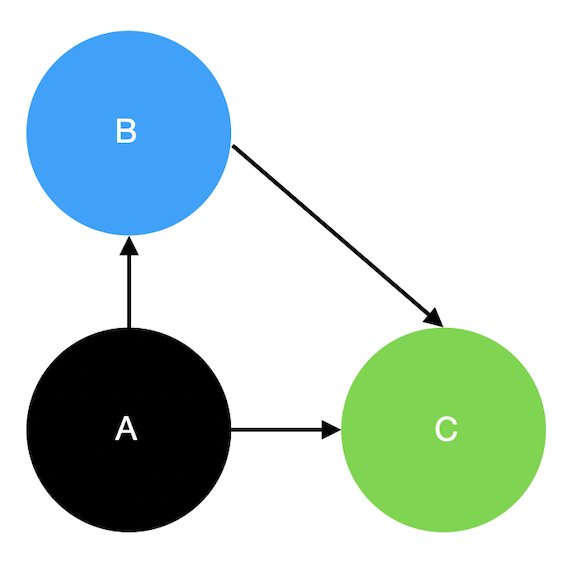
\includegraphics{img_08.png}
\end{frame}

\begin{frame}{Database Interaction}
    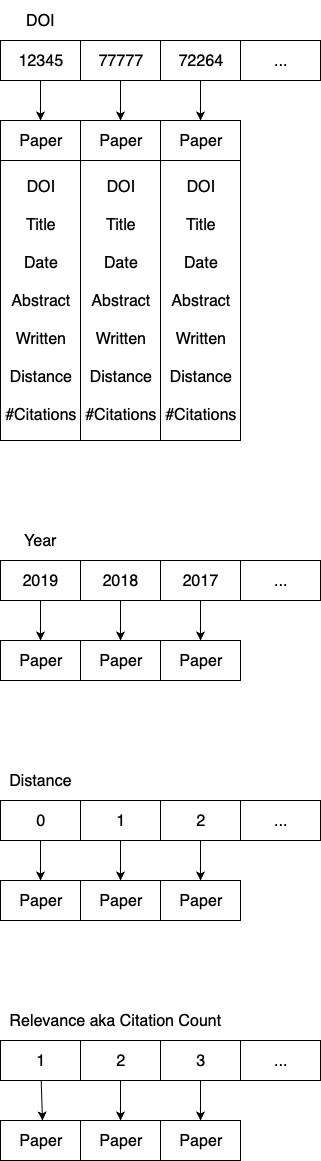
\includegraphics{img_09.png}
\end{frame}

\begin{frame}{Responsiblities}
    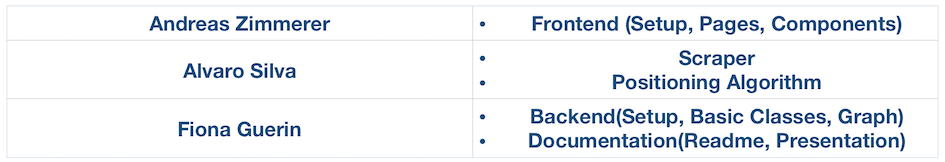
\includegraphics{img_10.png}
\end{frame}

\begin{frame}{Lessons Learned: Plan}
    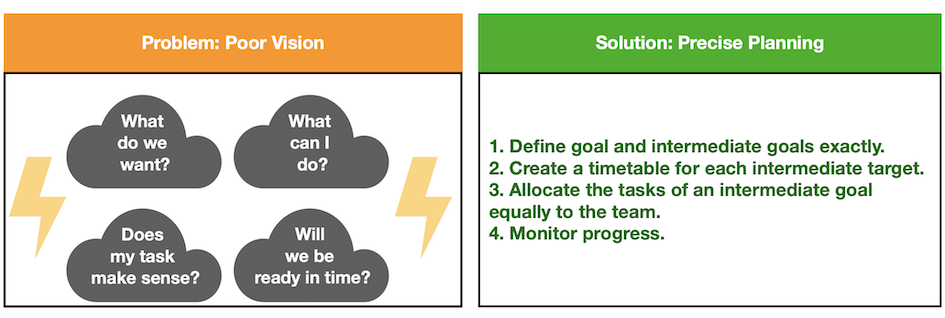
\includegraphics{img_11.png}
\end{frame}

\begin{frame}{Lessons Learned: Communicate}
    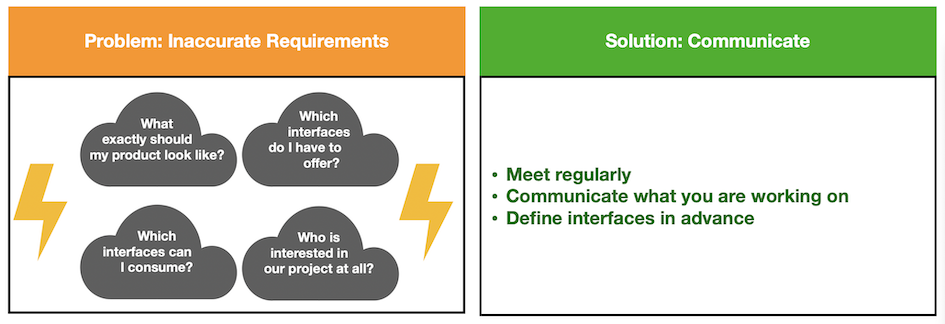
\includegraphics{img_12.png}
\end{frame}

\begin{frame}{Github}
    \url{https://github.com/Jibbow/research-paper-graph}
\end{frame}

\begin{frame}{Thank you}
    
\includegraphics{img_05.png}
\end{frame}

\end{document}
